The \textit{test data} module is responsible for management and cataloguing of
test data to be used in the benchmarking tests.

\subsection{Scope}
The scope for the test data module is shown in Figure \ref{fig:testData}
\begin{figure}[H]
  \begin{center}
  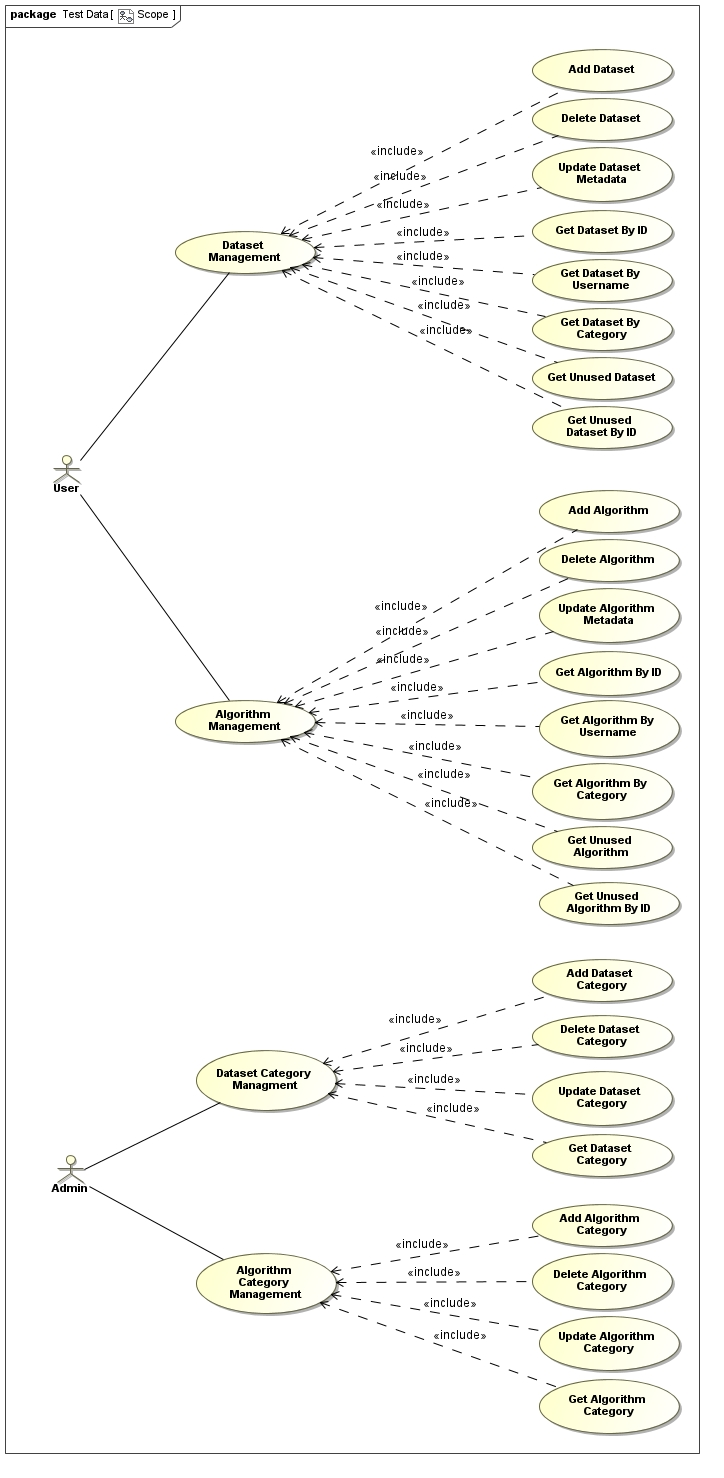
\includegraphics[scale=0.7]{../Diagrams and Charts/Test Data/Scope.jpg}
  \caption{Test Data}
  \end{center}
  \label{fig:testData}
\end{figure}
The scope of the test data module include:
\begin{itemize}
	\item The user can dynamically generate test data
	\item Users can rate dynamic or user upload data sets
	\item Any user can upload there own dataset to the growing repository of data sets 
	\item Users will be able to view the data set with associated meta data
\end{itemize}

\subsection{Domain Model}
The domain model for the test data module is shown in Figure \ref{fig:testDataModel}
\begin{figure}[H]
  \begin{center}
  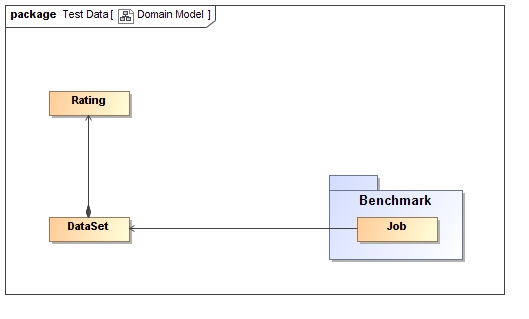
\includegraphics[scale=0.5]{../Diagrams and Charts/Test Data/Domain Model.jpg}  
  \caption{Test Data Domain Model}
  \end{center}
  \label{fig:testDataModel}
\end{figure}
